\documentclass[11pt,a4paper]{article}

% These are extra packages that you might need for writing the equations:
\usepackage{amsmath}
\usepackage{amsfonts}
\usepackage{amssymb}
\usepackage{booktabs}
\usepackage{hyperref}
\usepackage{listings}
\usepackage{xcolor}
\usepackage{outlines}
\usepackage{mathtools}

\lstset {language=C++,
		 basicstyle=\ttfamily,
         keywordstyle=\color{blue}\ttfamily,
         stringstyle=\color{red}\ttfamily,
         commentstyle=\color{purple}\ttfamily,
         morecomment=[l][\color{magenta}]{\#},
       	 basicstyle=\tiny}

% You need the following package in order to include figures in your report:
\usepackage{graphicx}

% With this package you can set the size of the margins manually:
\usepackage[left=2cm,right=2cm,top=2cm,bottom=2cm]{geometry}


\begin{document}

% Enter the exercise number, your name and date here:
\noindent\parbox{\linewidth}{
 \parbox{.25\linewidth}{ \large ICP, Exercise 09 }\hfill
 \parbox{.5\linewidth}{\begin{center} \large Beat Hubmann \end{center}}\hfill
 \parbox{.2\linewidth}{\begin{flushright} \large Nov 25, 2018 \end{flushright}}
}
\noindent\rule{\linewidth}{2pt}


\section{Introduction}

Both the Newton-Raphson method and the Secant method were implemented and employed
to find an extremum of a continuous multivariate function. If started on a point close
enough to the extremum, both (very similar) methods were found to converge on the maximum
which was known analytically in the case under consideration.

\section{Algorithm Description}
While the algorithm as such is quite simple, using it on the given function $F(x, y) = e^{-(x - x_0)^2 -(y -y_0)^2}$ requires
some setup.\\
Analogous to the univariate case, to find the (global) maximum of $F(x,y)$, we must find the root of $\vec{\nabla} F(x, y)$,
or in other words, the solution of $ \vec{0} = \vec{f}(x,y) \coloneqq \vec{\nabla}F(x,y)$ (see equation~\ref{eqn:1}).
The Jacobi matrix of $f(x,y)$ required by the Newton-Raphson method then is as described
by equation~\ref{eqn:2}.


\begin{equation}
	\begin{pmatrix}
		0 \\
		0 
	\end{pmatrix}
	=
	\vec{f}(x,y) \coloneqq 
	\begin{pmatrix}
		\partial F(x,y)/\partial x \\
		\partial F(x,y)/\partial y
	\end{pmatrix}
	=
	\begin{pmatrix}
		-2(x-x_0) \cdot e^{-(x - x_0)^2 -(y -y_0)^2} \\
		-2(y-y_0) \cdot e^{-(x - x_0)^2 -(y -y_0)^2}
	\end{pmatrix}
	\label{eqn:1}
\end{equation}


\begin{equation}
	\begin{array}{lll}
	\vec{\vec{J}}_f(x,y)
	& =
	\begin{pmatrix}
		\partial f_x(x,y)/ \partial x & \partial f_x(x,y)/ \partial y \\
		\partial f_y(x,y)/ \partial x & \partial f_y(x,y)/ \partial y \\
	\end{pmatrix}
	 =
	\begin{pmatrix}
		\partial^2 F(x,y) / \partial x^2 & \partial^2 F(x,y) / \partial x \partial y \\
		\partial^2 F(x,y) / \partial y \partial x & \partial^2 F(x,y) / \partial x^2 
	\end{pmatrix}
	= \\
	& =
	e^{-(x - x_0)^2 -(y -y_0)^2} \cdot  
	\begin{pmatrix}
	4(x - x_0) - 2 & 4(x-x_0)(y-y_0) \\
	4(x - x_0)(y - y_0) & 4(y - y_0)^2 - 2	
	\end{pmatrix}
\end{array}
	\label{eqn:2}
\end{equation}

For brevity, we refer to the task description for the interpolating Jacobian of 
the Secant method.

With the only difference between the Newton-Raphson method and the Secant method
being the way the Jacobian matrix is calculated, the algorithm then works as follows:
\begin{outline}
\1 Choose starting point $\vec{x}_0$ close enough to suspected maximum
\1 While $f(x_{n+1}) > \epsilon$
	\2 Do $\vec{x}_{n+1} = \vec{x}_n - (\vec{\vec{J}}_f(\vec{x}_n))^{-1} \cdot f(\vec{x}_n)$
\1 Output $\vec{x}_{n+1}$
\end{outline}
\section{Results}

The program was implemented as described above and submitted with this report. 
For the given problem, the Jacobian matrices of the methods are almost equal,
and both were found to converge for starting values $x,y$ in the range $x \in [x_0 - \xi, x_0 + \xi ], y \in [y_0 - \upsilon, y_0 + \upsilon]; \quad \xi=\upsilon=0.35$ 
(see figures~\ref{fig:1}~and~\ref{fig:2}).

\begin{figure}[ht]
\begin{center}
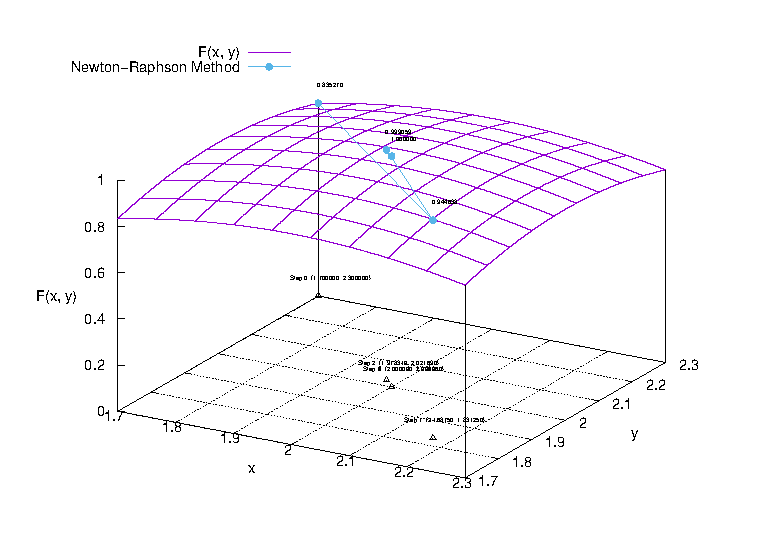
\includegraphics[scale=1.2]{figure1.eps} 
\end{center}
\caption{Convergence steps of Newton-Raphson method to find maximum of $F(x,y)=e^{-(x - x_0)^2 -(y -y_0)^2}; x_0=y_0=2$.}
\label{fig:1}
\end{figure}

\begin{figure}[ht]
\begin{center}
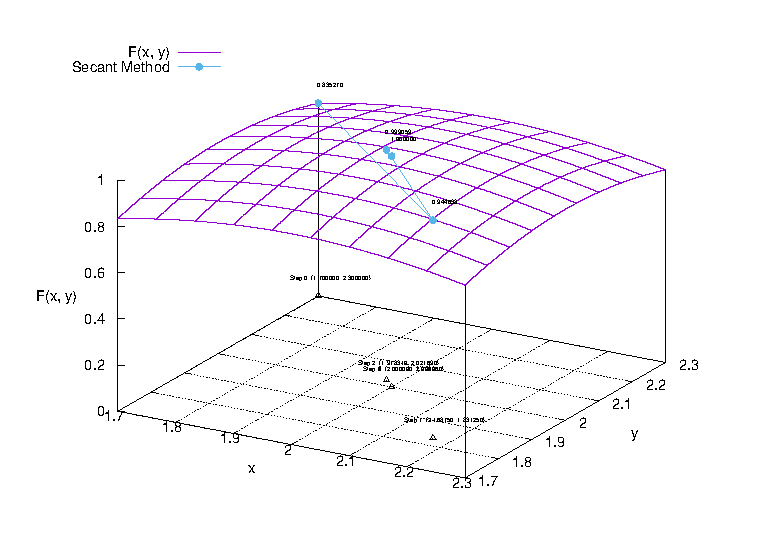
\includegraphics[scale=1.2]{figure2.eps} 
\end{center}
\caption{Convergence steps of Secant method to find maximum of $F(x,y)=e^{-(x - x_0)^2 -(y -y_0)^2}; x_0=y_0=2$.}
\label{fig:2}
\end{figure}

\section{Discussion}
Both methods were found to converge in an equal amount of steps. As expected, 
the starting coordinates have to be chosen close to the actual maximum for the methods
to converge.
% \begin{thebibliography}{99}


% \bibitem{metropolis}
% Metropolis, N.,
% Rosenbluth, A.W.,
% Rosenbluth, M.N.,
% Teller, A.H.,
% Teller, E.\\
% \emph{Equations of State Calculations by Fast Computing Machines},\\
% Journal of Chemical Physics. 21 (6): 1087,\\
% 1953.


% \bibitem{herrmann}
% 	Herrmann, H. J.,
% 	Singer, H. M.,
% 	Mueller L.,
% 	Buchmann, M.-A.,\\
% 	\emph{Introduction to Computational Physics - Lecture Notes},\\
% 	ETH Zurich,\\
% 	2017.


% \end{thebibliography}

\end{document}